\documentclass[tikz,border=5pt]{standalone}
\usepackage{amsmath,amssymb}
\begin{document}
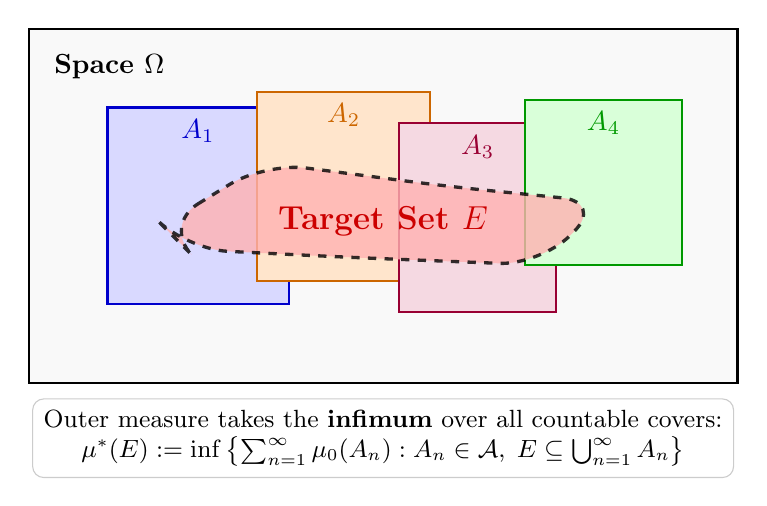
\begin{tikzpicture}[>=latex, font=\small]
  % Space Omega
  \draw[thick, fill=gray!5] (-0.5, -0.5) rectangle (8.5, 4.0);
  \node[anchor=north west, font=\bfseries] at (-0.3, 3.8) {Space $\Omega$};

  % Sets A_n covering E
  \draw[thick, fill=blue!15, draw=blue!80!black] (0.5, 0.5) rectangle (2.8, 3.0);
  \node[blue!80!black, font=\bfseries] at (1.65, 2.7) {$A_1$};

  \draw[thick, fill=orange!20, draw=orange!80!black] (2.4, 0.8) rectangle (4.6, 3.2);
  \node[orange!80!black, font=\bfseries] at (3.5, 2.9) {$A_2$};

  \draw[thick, fill=purple!15, draw=purple!80!black] (4.2, 0.4) rectangle (6.2, 2.8);
  \node[purple!80!black, font=\bfseries] at (5.2, 2.5) {$A_3$};

  \draw[thick, fill=green!15, draw=green!60!black] (5.8, 1.0) rectangle (7.8, 3.1);
  \node[green!60!black, font=\bfseries] at (6.8, 2.8) {$A_4$};

  % Arbitrary set E
  \draw[very thick, dashed, fill=red!30, opacity=0.8] 
    (1.2, 1.5) [rounded corners=15pt] -- (2.5, 2.3) -- (4.8, 2.0) -- (6.8, 1.8) 
    -- (6.0, 1.0) -- (3.5, 1.1) -- (1.5, 1.2) -- cycle;
  \node[font=\large\bfseries, red!80!black] at (4.0, 1.55) {Target Set $E$};

  \node[align=center, fill=white, draw=gray!40, rounded corners, inner sep=4pt] at (4.0, -1.2)
    {Outer measure takes the \textbf{infimum} over all countable covers:\\
     $\mu^*(E) := \inf \left\{ \sum_{n=1}^\infty \mu_0(A_n) : A_n \in \mathcal{A},\; E \subseteq \bigcup_{n=1}^\infty A_n \right\}$};
\end{tikzpicture}
\end{document}
